\chapter{Final Tool and Launch}

This chapter will detail the final iteration of the VCWiz platform, and our efforts to launch it to the public.

\section{Final VCWiz Interface}

The final platform incorporated all the feedback from previous iterations, and was built over a span of four months. Below, we detail the technical details of the platform's interface, exploring each aspect in the order a new user would.

\subsection{Onboarding}

Founders find the VCWiz platform through one of our launch partners (such as TechCrunch\footnote{\url{https://techcrunch.com/2018/01/25/dorm-room-fund-has-built-a-crm-for-founders-raising-a-seed-round/}}), or from search engines such as Google. We spent the months leading up to the launch generating research pages for every investor, firm, and company in our database. These pages include comprehensive details on the entity in question, as described above, as well as an embedded view of all the VCs associated with that entity, and, if the user is signed in, all the personalization included in the platform.

\begin{figure}[ht]
  \centering
  \begin{minipage}{0.45\textwidth}
    \centering
    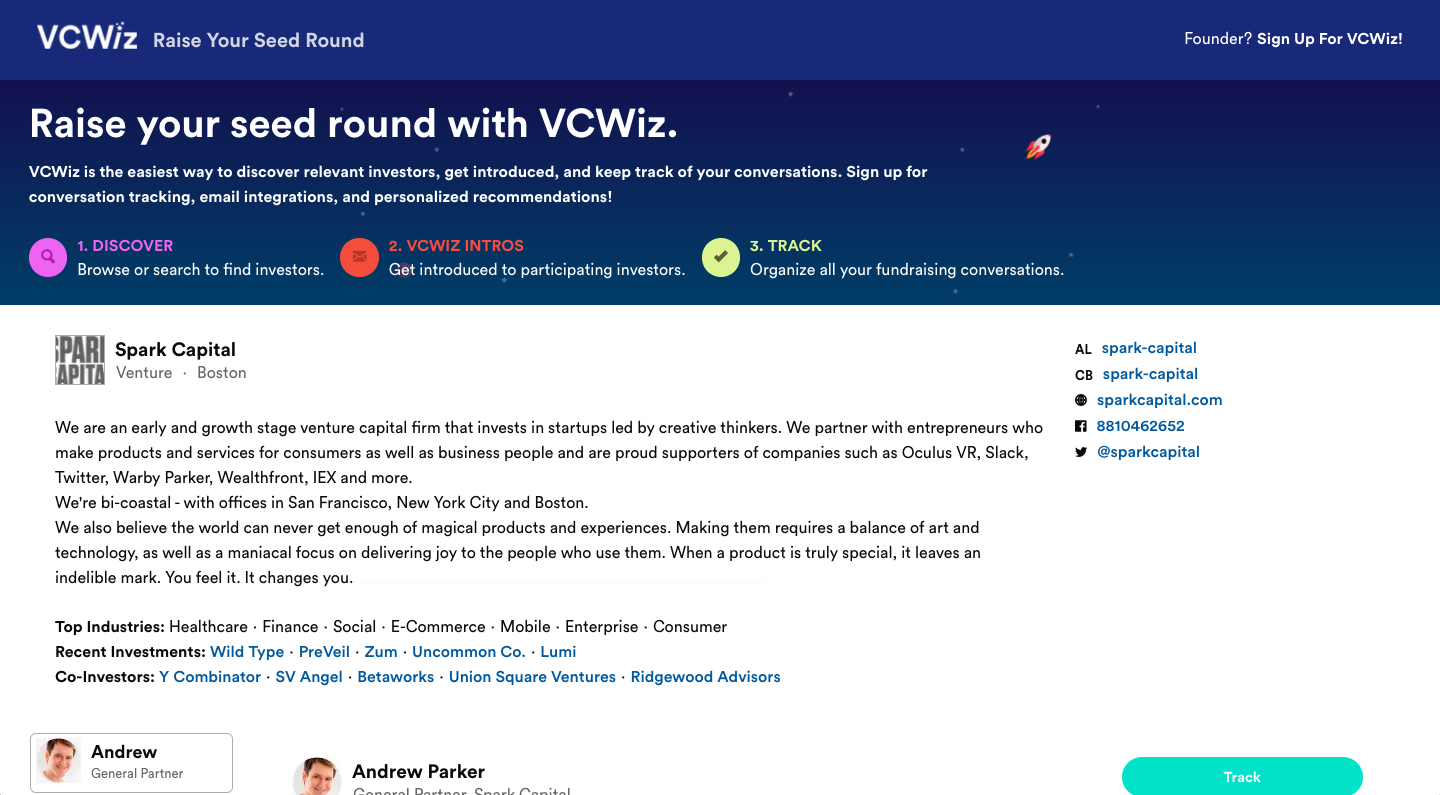
\includegraphics[width=0.9\textwidth]{vcwiz/onboarding/firm.png}
    \caption*{Spark Capital Firm Page}
  \end{minipage}\hfill
  \begin{minipage}{0.45\textwidth}
    \centering
    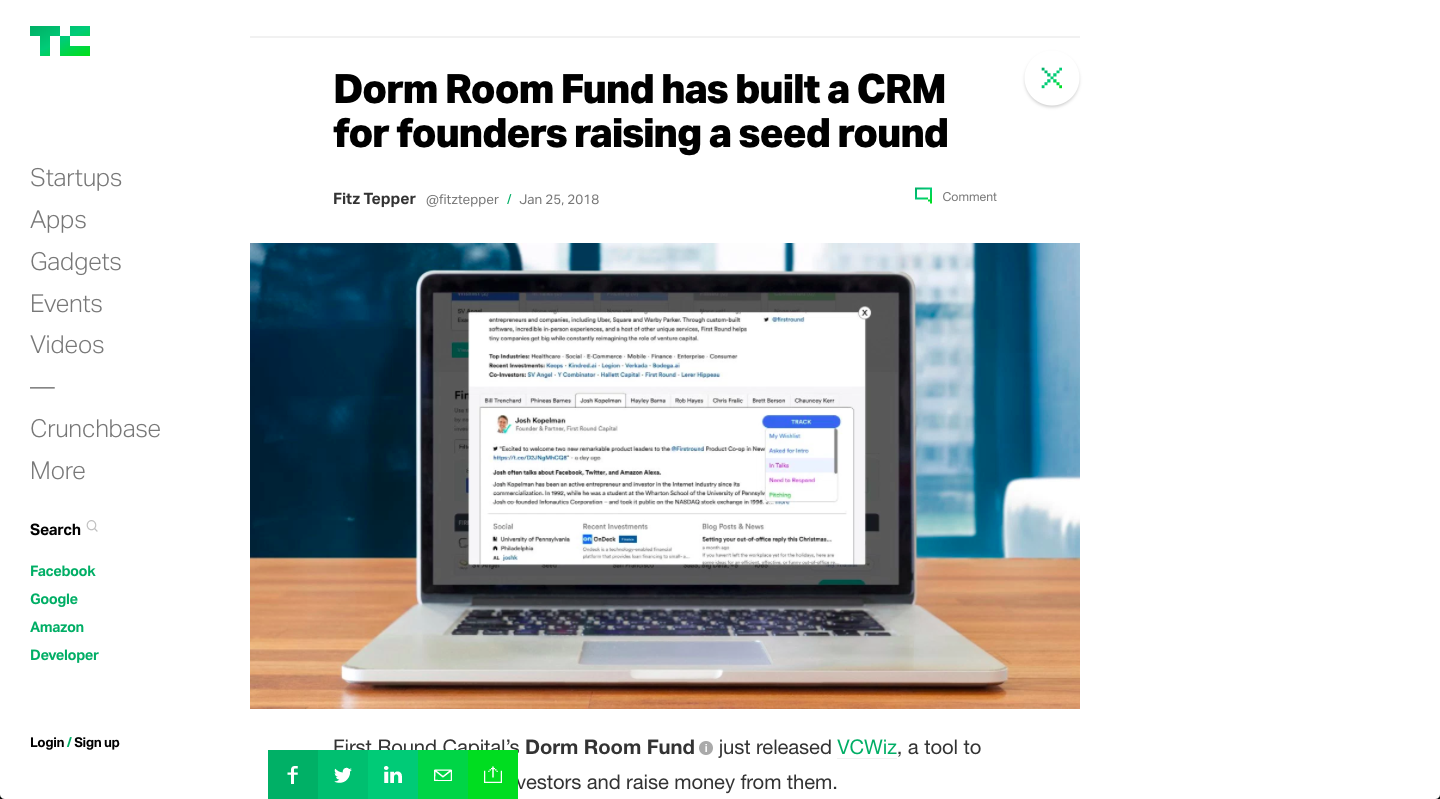
\includegraphics[width=0.9\textwidth]{vcwiz/onboarding/techcrunch.png}
    \caption*{Launch on TechCrunch}
  \end{minipage}
\end{figure}

After funneling users from their landing page to the main screen of the application, founders are able to filter, search, and explore lists of investors without creating an account. The site is fully functional from a discovery and research perspective, and about 80\% of users are content to peruse the content without creating an account. If the founder decides to create an account, we walk them through a series of questions to gather more information about their startup.

\begin{figure}[ht]
  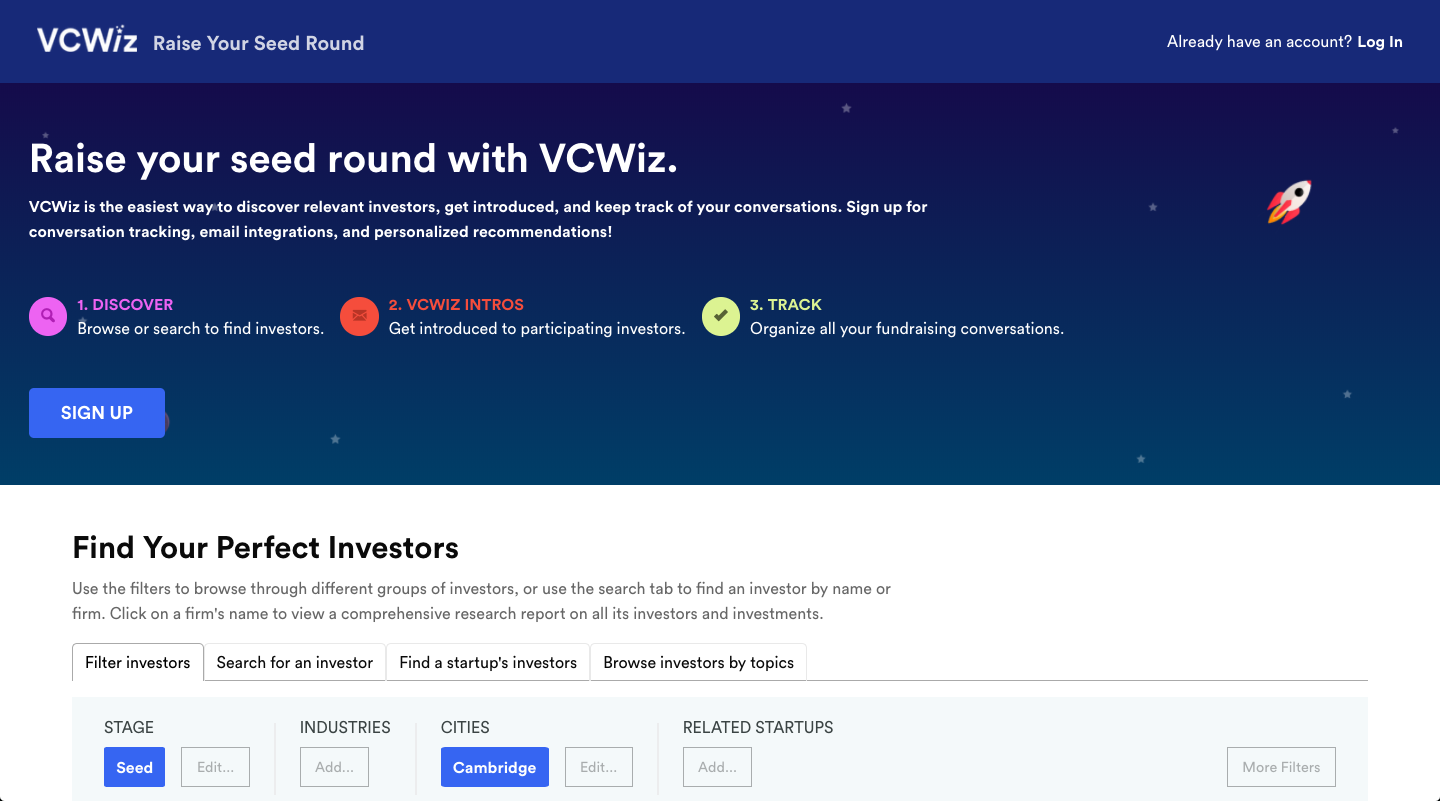
\includegraphics[width=0.45\textwidth]{vcwiz/onboarding/landing.png}
  \centering
  \caption*{VCWiz Landing Page}
\end{figure}

The signup flow begins by asking for the domain of the company. Using this as a unique identifier, we are able to query both our internal database, as well as external services (such as the Clearbit Logo API \footnote{https://clearbit.com/logo}) to gather as much information as possible on the founder's startup. The client browser makes a request to an API backend on the VCWiz server which initiates these requests in parallel, and returns a joined \texttt{Company} model within a given timeout threshold. This information is used pre-fill many of the following fields, including the name, description, industries, and competitors of the company. The founder is given a chance to verify this information, as well as provide mandatory information on their ideal investor profile. Finally, the founder is requested to log in with their Google account, in order to provide an authenticated email and social profile. We chose to use an OAuth2 \cite{hardt2012oauth}-based login flow with an existing service provider to simplify the login experience, and to avoid having to store user credentials. Google was the platform of choice on account of it providing verified email address information to users, as well as to unify the authentication experience in the case that the founder also decides to provide API access to their email inbox (for the purpose of synchronizing their conversations with investors).

Providing access to their email inbox is strictly an opt-in feature, and the how the data is to be used is explicitly described. As a result of our surveys to founders in previous iterations of the product, we found that it was necessary to have a plain-English description of our data use policy. We guarantee to founders that no human will ever read the individual messages of their inbox, that only aggregate data will be used for purposes other than their personal dashboard, and that we will only use metadata from their emails (headers, sentiment, etc.).

After signing up, the founder is presented with a brief set of video clips that introduce the functionality to them, including how to filter, search, and track investors. Following this, the site functions as it did before the founder signed up, with a few minor changes. Every screen with an investor has an integrated conversation tracker which shows the status of that investor, if any, in the founder's fundraise, as well as the email-based shortest intro path to that investor. The results of the filters are also personalized to the founder, based on the overlap in industries and location between each firm and the founder's startup. Signing up also unlocks the conversation tracker, with a preview of conversations on the main page, and a dedicated screen for updating and viewing the status of each individual conversation.

\begin{figure}[ht]
  \centering
  \begin{minipage}{0.33\textwidth}
    \centering
    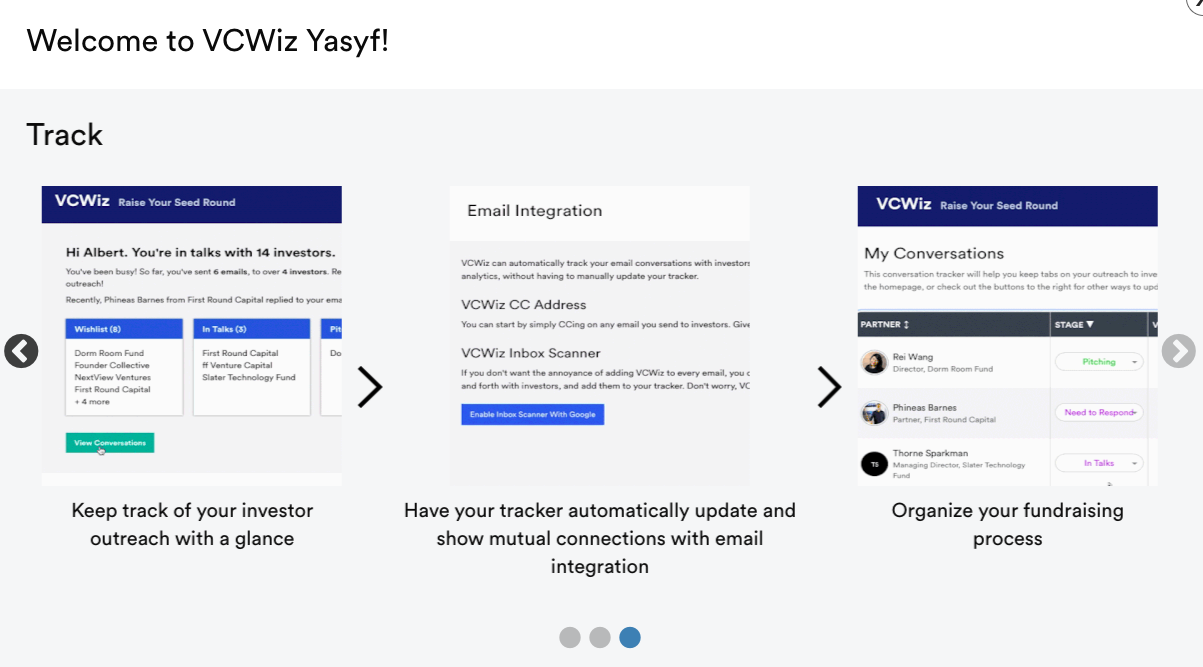
\includegraphics[width=0.9\textwidth]{vcwiz/onboarding/intro.png}
    \caption*{Tutorial}
  \end{minipage}\hfill
  \begin{minipage}{0.33\textwidth}
    \centering
    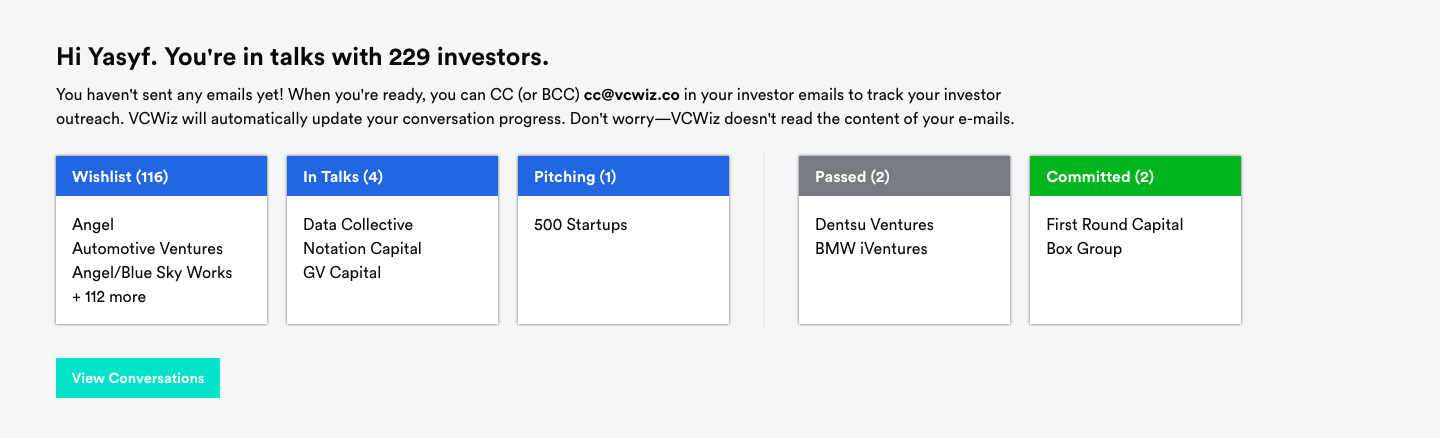
\includegraphics[width=0.9\textwidth]{vcwiz/onboarding/summary.png}
    \caption*{Conversation Summary}
  \end{minipage}\hfill
  \begin{minipage}{0.33\textwidth}
    \centering
    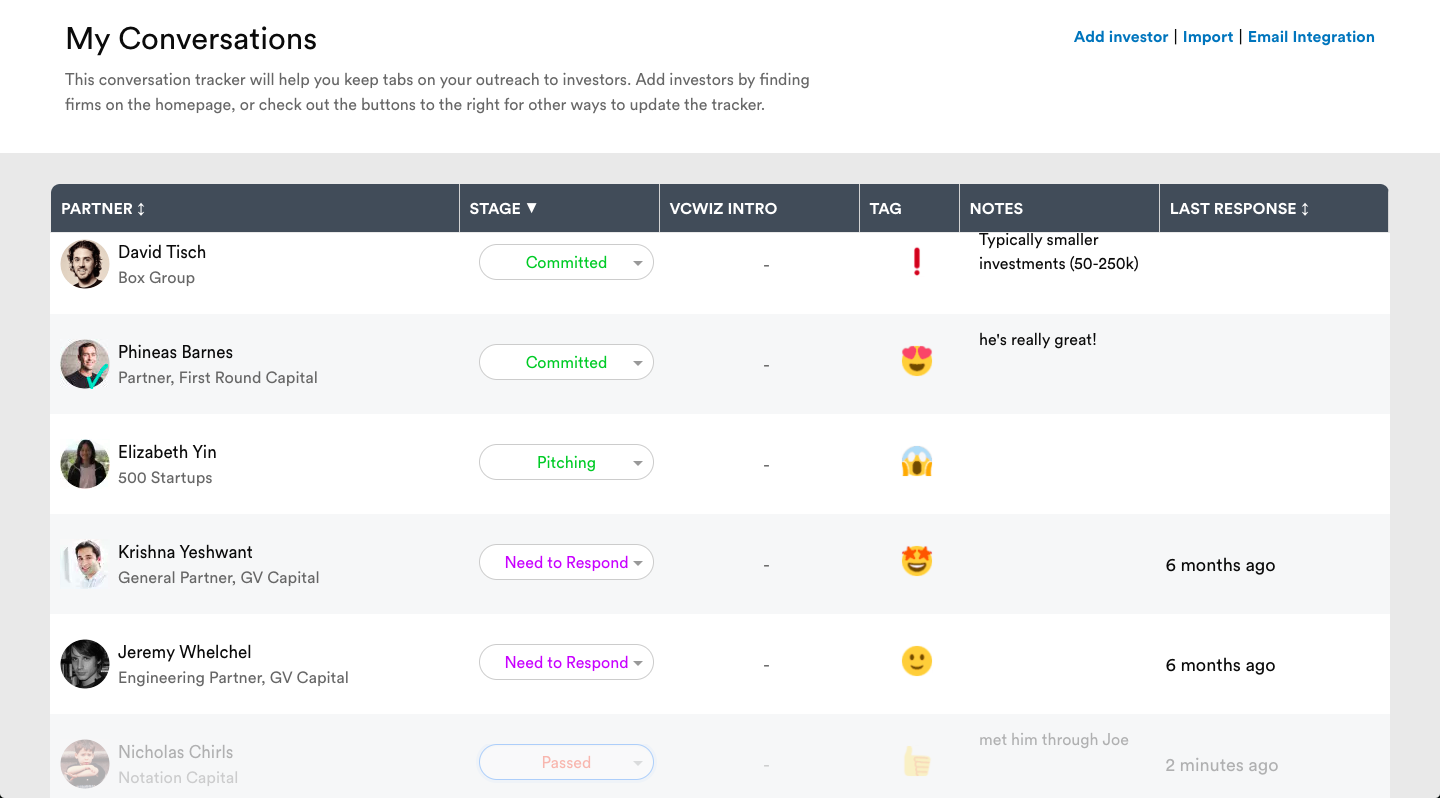
\includegraphics[width=0.9\textwidth]{vcwiz/onboarding/conversations.png}
    \caption*{Conversation Tracker}
  \end{minipage}
\end{figure}

\subsection{Ingesting User Data}
\label{vcwiz:ingesting}

One of the major insights from previous iterations of VCWiz was that founders have a variety of different ways they create and interact with data about their fundraising process, and they aren't often willing to change those. Thus, the tool we built had to meet founders wherever they currently were, in order to get their conversation tracker on our platform caught up. We built three independent tools for letting the system know about ongoing conversation, in addition to the integrations in the research and discovery sections.

The first (and easiest) way founders can import their conversations to the platform is to grant access to their Gmail inbox, either during the signup flow or when later prompted. This allows a regularly-scheduled job on our server to poll an API offered by Google \footnote{https://developers.google.com/gmail/api/}, and import new messages according to the pseudocode in Listing \ref{code:sync}. A \texttt{history\_id} parameter is cached in the \texttt{Founder} model to indicate the most recent thread fetched from Google, to avoid fetching duplicates in the future.

\begin{lstlisting}[float,frame=single,mathescape=true,language=Ruby,basicstyle=\footnotesize,columns=fullflexible,caption={Sync Inbox},label={code:sync}]
def sync_inbox(founder):
  for thread in fetch_threads(founder.address, founder.history_id):
    messages $\gets$ thread.fetch_messages()
    for message in messages:
      if message.from == founder.address:
        parse_outgoing(founder, message)
      else:
        parse_incoming(founder, message)
    founder.history_id $\gets$ thread.id
\end{lstlisting}

Parsing messages follows the algorithm in Listing \ref{code:parse}, which also augments the founder's email-based graph with every email processed.

\begin{lstlisting}[float,frame=single,mathescape=true,language=Ruby,basicstyle=\footnotesize,columns=fullflexible,caption={Parse Message},label={code:parse}]
def parse_message(message):
  if check_if_bulk(message):
    return
  founder.graph.connect(message.address)
  target_investor $\gets$ find_or_create_target_investor(founder, message)
  if !target_investor:
    return
  if !target_investor.email:
    target_investor.email $\gets$ message.address
  target_investor.stage $\gets$ guess_stage(message)
  create_new_email(founder, target_investor, message)
\end{lstlisting}

As can be seen from the algorithm, when importing a user's emails and creating their email graph, we first started with the naive approach of scanning every email, creating a node (if one did not already exist) per address, and creating outgoing edges every time one node sent an email to another. While this works when only importing emails once, the APIs at our disposal were imperfect. The \texttt{history\_id} tracked from Google's API often expire, and imports must be repeated. Thus, we had to start tracking a unique message identifier in our own database to ensure emails are imported at most once.

There were also several heuristics we used to skip messages that could be classified as bulk mail, as this added a lot of noise to the dataset. If the message meets any of the following criteria, it is logged and skipped. The full algorithm can be found online \footnote{https://git.io/vxunk}. In these criteria, the recipients are defined as the union of the TO, CC, and BCC fields, and body is defined as the concatenation of the text and HTML sections of the message.

\begin{itemize}
  \item There are more than 5 recipients
  \item The body contains a phrase often used in bulk mailings, such as ``unsubscribe'', ``terms of use'', or ``view in your browser''
  \item The headers contain one of several common listserv headers, such as List-Unsubscribe and many vendor-specific ones
  \item The return path of the message includes a popular bulk email vendor
  \item The local component of the from address is that of a commonly-automated inbox, such as ``noreply'' or ``info''
  \item The name of the sender includes common aliases, such as ``support'' or ``payroll''
  \item The domain of the sender or any recipient is one that is common in transactional emails
\end{itemize}

The second way founders can inform the system about ongoing conversations is to CC (or BCC) a special email address, which routes to a server which accepts the message and forwards the relevant metadata to an API endpoint on VCWiz. This metadata is parsed and the email is reconstructed, before being run through the same algorithms as above. This alternate, manual way of updating VCWiz via emails was added for the more privacy-conscious founders on the platform, who wished to have the convenience of updates based on emails without handing over access to their entire inbox.

The third and final ways founders can update the system in bulk is by uploading a existing spreadsheet of conversations. Our surveys revealed that the most commonly-used tool for tracking conversations with an investor was a spreadsheet (or spreadsheet-like tool), so providing an easy way to migrate those onto the platform was essential. Founders can export a CSV file from any spreadsheet-based tool and import it on the conversation tracker page of VCWiz. The server parses the rows out of the CSV, and uses both the format of the content of a column as well as it's header (based on the Levenshtein distance \cite{1966SPhD...10..707L} of a given header from a list of common choices) to guess which columns correspond to which internal database columns of a \texttt{TargetInvestor}. This mapping is presented to the founder for verification, and then is used to import the rows as a background job.

\begin{figure}[ht]
  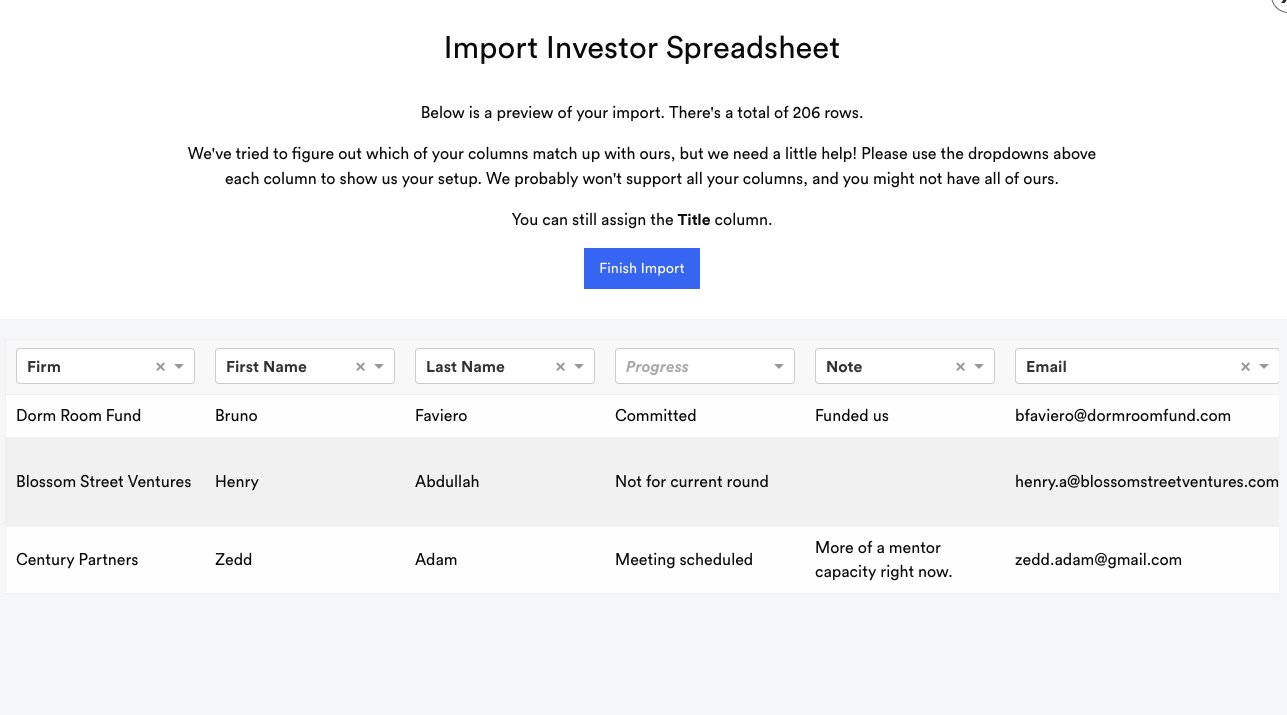
\includegraphics[width=0.45\textwidth]{vcwiz/import/columns.png}
  \centering
  \caption*{Spreadsheet Import}
\end{figure}

\subsection{Filtering \& Searching}

\subsubsection{Filtering}

The main filtering interface of VCWiz allows founders to display investors that match a set of criteria. We will detail each of those criteria before describing the algorithm used to filter. The logic behind the selection of criteria is to cover the majority of the ways founders describe their ideal investor: the stage the investor operates at, the industries that they invest in, the location they invest in, and their relationship to similar/competing companies (similar companies are generally a good sign, whereas directly competing companies might be prohibitive).

The first criteria is based on the stage of the company, as defined by it's latest funding round. It is a filter on the funding round a venture fund invests in, either as reported by the fund, or based on their past investments. Note that a fund can have multiple stages affiliated with it, as can a funding round of a company (often in the cases of ambiguity); when aggregating past investments, any stage which shows up at least half of the time is attributed to the fund. This criteria is always a logical \texttt{OR} when multiple are selected.

The next criteria is the set of industries that a fund commonly invests in. Once again, these are preferably self-reported, and there can be multiple associated with a fund (as well as an investor or a company). They are aggregated in the same was as the stage. The set of industries are fixed: there is no free-form option when filtering. The set of industries to display as options \footnote{https://git.io/vpTbj} was selected using the algorithm in Listing \ref{code:industries}, on all the companies in the Crunchbase data set. The goal is to select the set of industries that cover the entire set, with minimal overlap.

\begin{lstlisting}[float,frame=single,mathescape=true,language=Ruby,basicstyle=\footnotesize,columns=fullflexible,caption={Display Industries},label={code:industries}]
def covering_industries(companies):
  all_industries $\gets$ companies.flat_map(c $\to$ c.industries)
  industry_options $\gets$ all_industries.unique()
  sorted_options $\gets$ industry.sort_by(i $\to$ all_industries.count(i))

  selected $\gets$ set()
  while companies.filter(c $\to$ c.industries $\cap$ selected $\neq \emptyset$).count() > 0:
    selected $\gets$ selected $\cup$ {sorted_options.pop()}

  return selected
\end{lstlisting}

By default, when a founder selects multiple industries, the filter is a logical \texttt{OR} of these industries. However, there is an option which can be toggled to make this filter an \texttt{AND}, such that returned companies have to invest in \textit{all} the specified industries.

The next criteria is based on a set of cities. By default, this filter returns firms which are based in the cities specified (firms have a single headquarters, and an array of locations, which are both matched against). There is an option, however, to change this filter to instead return firms that have invested in \textit{startups} based in the specified city (each startup is affiliated with a single city).

Another criteria to be matched against is a set of relevant startups. The founder can select this set from the database of companies VCWiz tracks internally. By default, this set restricts the returned firms to those who have invested in at least one of the specified companies. An option can be toggled which changes this filter to restrict to the set of firms that have invested in \textit{similar} companies, based on the industries of each company in the set.

The final criteria to match investors against is a set of topics. In this case, a topic is anything found in the VCWiz entity database, built up by extracting entities from the various data sources discussed elsewhere. At the time of writing, this database contains $98,000$ records. The filter based on these entities is a logical \texttt{OR}, and will return investors who often mention or discuss any of the given topics. In this case, we include a topic for an investor if that topic is mentioned at least 5\% of the time in content created by or mentioning the investor.

Finally, here is a lone option to restrict the returned set of investors to those that operate solely in the US. This was a popular criteria for many founders on our platform.

\subsubsection{Searching}

In addition to filtering against any combination of the above criteria, founders can also filter investors based on the name of the firm or individual investor. This is implemented as a simple fuzzy string match on the \texttt{name} field of \texttt{Firm}, and the \texttt{first\_name} and \texttt{last\_name} fields of \texttt{Investor}.

\subsubsection{Sort}

Once VCWiz have generated the set of investors that match each filter and search query, it must decide the order in which to display the results. There is a custom ranking function which sorts the results, using each metric as the tie-breaker for the last.

\begin{enumerate}
  \item If the topic filter is present: the number of investors in the firm which match the set of topics
  \item The number of ``featured'' investors in the firm
  \item If the industry filter is present: the number of intersecting industries between the firm and the query
  \item If the city filter is present: the number of intersecting cities between the firm and the query
  \item The number of founders on the platform who have initiated a conversation with the firm
  \item The number of ``verified'' investors in the firm
\end{enumerate}

N.B. Any metric which does not have it's requirement met is simply ignored. ``Featured'' investors are those on the platform who have been hand-picked as high-quality investors. ``Verified'' investors are those who have completed their investor profile on VCWiz self-reported their characteristics.

This sort achieves personalization by using the industries of the founder's startup and current location of the founder for the purpose of sorting, when the respective filters for those characteristics are not specified. Thus, if a founder specifies all the possible filters, they will get the same results that any other founder who does the same will. However, if the relevant filters are unspecified, information from the founder's profile will be used for ranking and displaying the results, giving a different ranking than some other founder.

The interface displayed to the founder also allows for manual sorting of the results based on the natural ordering of a given column. If this overriding sort is provided, none of the above is used.

\subsubsection{Implementation}

The algorithm for displaying the results of this process \footnote{https://git.io/vpkvd} is demonstrated in Listing \ref{code:filter}.

We start with every firm in the database, and filter out any that do not match the search terms provided by the founder. Often, the search term is given as a single query string. In this case, we treat this string as both the query for the firm name, as well as the investor name (the first word of the string is considered the query for the first name, and the remainder for the last name). Any individual investors who match have their firms added to the results.

Following the search query, we apply every present filter to the remaining set of firms, narrowing down the result set each time.

\begin{lstlisting}[float,frame=single,mathescape=true,language=Ruby,basicstyle=\footnotesize,columns=fullflexible,caption={Filter and Search},label={code:filter}]
def filter_and_search(all_firms, founder, filters, search):
  firms $\gets$ all_firms
  investors $\gets$ firms.flat_map(f $\to$ f.investors)

  if search:
    first_name, last_name = extract_name_components(search)
    investor_by_name $\gets$ investors.filter(i $\to$
      i.first_name.contains(first_name) || i.last_name.contains(last_name)
    )
    firms_by_investor_name $\gets$ investor_by_name.map(i $\to$ i.firm)
    firms_by_name $\gets$ firms.filter(f $\to$ f.name.contains(search))
    firms $\gets$ firms_by_name $\cup$ firms_by_investor_name

  for filter in filters:
    firms $\gets$ apply_filter(firms, filter)

  sorted $\gets$ apply_ordering(firms, founder, filters)
  return sorted
\end{lstlisting}

\subsubsection{Display}

The results from the filtering and searching process are displayed in an infinitely-scrollable table to the founder, with the following columns.

\begin{enumerate}
  \item The name and photo of the firm
  \item The company stages the firm invests at
  \item The headquarters of the firm
  \item The number of investments the firm has made in the last calendar year (``pace'')
  \item The top three industries that the firm invests in
  \item A drop-down to add or update the firm in the conversation tracker
\end{enumerate}

N.B. What founders really desire to see in the ``stage'' column is the average cheque size of the firm. However, this number is difficult if not impossible to calculate given the limited public data on investor contributions to a given fundraising round. Thus, the company stage is used as a proxy.

The ``pace'' column is present to give the founder a sense of how active a given firm is. This was added by popular request after many founders found it difficult to determine whether or not a firm was still actively investing their current fund.

\begin{figure}[ht]
  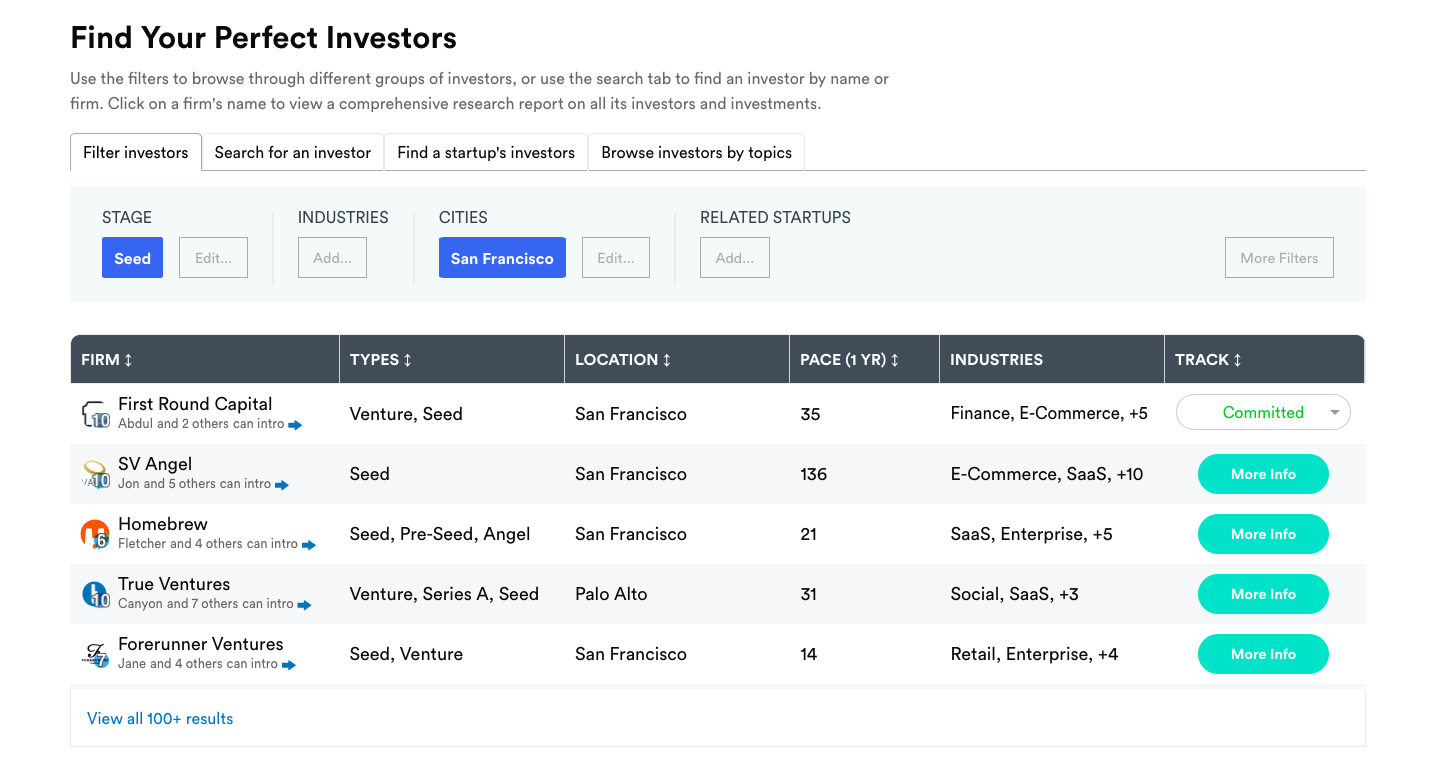
\includegraphics[width=0.45\textwidth]{vcwiz/filtering/results.png}
  \centering
  \caption*{Filter Results}
\end{figure}

Each column (other than ``industries'') also provides a button for overriding the ranking function. This allows the founder to view the result set, sorted by only the data in the particular column. The ``firm'' and ``location'' columns are sorted lexicographically, the ``pace'' column numerically, and the ``stage'' and ``track'' columns by their inherently-defined orderings.

In the case where a search query is specified, or the topic filter is used, it is valuable to not only surface not only the resulting firms, but the best-matching investor at each firm (e.g. if the search query matches the first name of a partner). In these cases, there is an additional, non-sortable column titled ``Partner'', which displays the name and photo of that best match.

\begin{figure}[ht]
  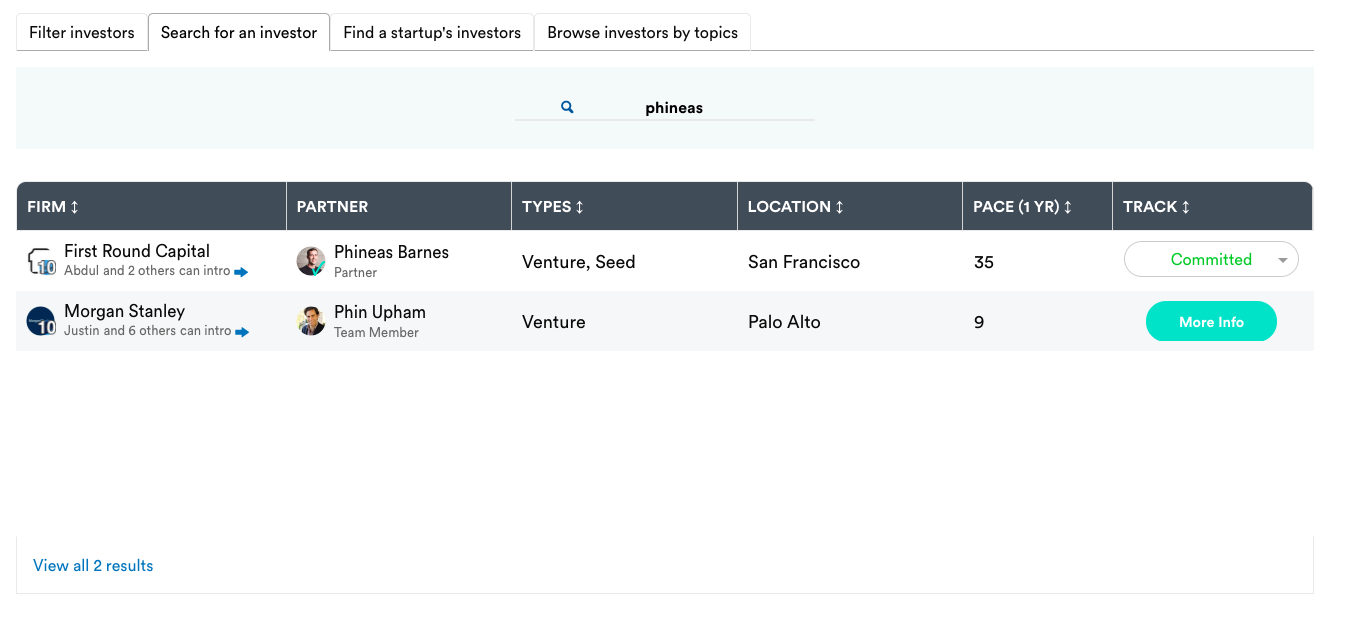
\includegraphics[width=0.45\textwidth]{vcwiz/filtering/partner.png}
  \centering
  \caption*{Filter Results with Partner Column}
\end{figure}

\subsubsection{Initialization}

When a founder first completes the signup flow for VCWiz, they are presented with a page containing functional real-time filtering, according to the above. To ensure a positive first experience viewing the results of filters, we make a few assumptions, and initialize the founder's filters to what we believe are sane defaults. We set the funding round filter to ``Seed'', to reflect the target user of the platform. The industry and relevant startups filters are pre-filled with the industry and competitors of the founder's startup, respectively. Finally, the location filter is set to the nearest ``hub city'', relative to the founder's current location (based on their IP address). A ``hub city'' is defined as a city that has at least 50 venture firm offices (as reported by VCWiz) within it.

\subsection{Introduction Requests}
\label{chap4:introrequests}

One experimental part of the final VCWiz platform was the ability for founders to request introductions to out-of-network investors on the platform.

The motivation behind this was to standardize the format and medium of ``cold'' intro requests in the venture community. As discussed earlier, there is both qualitative and quantitative data supporting the use of mutual connections to make introductions when reaching out to investors. This is corroborated by the results of our experiments on the VCWiz graph, which indicate that how central a founder is in the global social graph of startups and venture capital is highly correlated with how easily a founder will raise money. However, sometimes this is simply not an option. In this case, founders resort to ad-hoc, unsolicited emails to investors, leveraging myriad folklore tactics to increase the chances of a response. This is a frustrating experience for both parties: investors are deluged with a stream of unwanted pitches, mixed haphazardly into their daily business, while founders are disappointed that their carefully-crafted custom email gets lumped in with the bulk email another founder sent to 1000 investors.

We attempted to solve this problem by providing a tool for founders to send a templated introduction request, which looks identical each time (save for a customizable blurb), to an investor. The investor's email address is never initially revealed to the founder. Instead, a request email is sent by the VCWiz platform to the investor, containing an automatically-generated dossier on the founder and their startup (from the information provided at signup). The investor can respond to this automated email with a simple ``yes'' or ``no'', and only in the case of an affirmative response is a second email sent from the platform, connecting the founder and the investor.

\textbf{\#TODO: images of request screen, email with options, eventual intro if they say yes}

While many investors agreed that using an automated third-party such as VCWiz was preferable to founders directly sending countless emails and followups, there was significant doubt that such a platform would be adopted to such a degree that it could be considered a success. As it turns out, these concerns were well-founded. When we launched the feature, we were tracking a funnel of four success metrics:

\begin{enumerate}
  \item The number of introductions requested
  \item The number of requests which receive a response
  \item The number of successful connections
  \item The number of investments made as a result of an introduction
\end{enumerate}

N.B. a ``successful connection'' is defined as any introduction which results in at least one additional email from each party.

A few months after launching the feature, we saw the following usage. Out of 301 introductions requested, only 19 garnered a response from the investor, of which five were affirmative. One of these resulted in a successful connection, and none resulted in an investment.

Our hypothesis was that this experiment failed for two reasons. The first was that the founders who resorted to using this tool were inexperienced at fundraising or were not very well-connected, which presents an adverse selection problem: as we will demonstrate later, founders who are not well-connected will struggle to raise relative to those who are. The second reason was that investors have such a low response rate to cold emails of any kind that any improvement was negligible.

We tested this hypothesis by surveying every founder on the platform, and every one of the 247 investors who had received an introduction request.

We asked the founders why they had or had not used the introduction request feature. 118 founders responded, with 10\% saying they had tried the feature, 23\% saying they would never get a cold introduction to an investor of any form, and 16\% not understanding the value of the feature. The long tail of remaining responses ranged from not currently needing any intros, to hitting bugs when trying to use the feature. This data supports that many founders are skeptical of using the feature, or any cold introduction, because of how ineffective they are. The majority of these founders (65\%) have exchanged emails with investors before, indicating they are the more seasoned founders.

Only 13 investors responded to the investor survey, but the overwhelming response was that the founders who had reached out were simply not high quality, or a good fit for their fund. This supports our hypothesis about founders, and the very fact that there were so few responses corroborates our hypothesis about investor response rates to unsolicited emails. An interesting corollary to a few of the responses was the realization that our solution still inconvenienced investors more than they would like. The ideal solution would involve a centralized dashboard of requests which could be checked for interesting prospects by designated individuals at the firm, often not the investors themselves.

\subsection{Intro Paths}

Founders who have shared their email graph with VCWiz can see their ``Intro Path'' to any given investor on the platform. The goal of displaying these paths (and the length of that path as investor's distance from the founder) is to assist founders in planning who can make an introduction for them (so as to avoid the problem discussed above).

\textbf{\#TODO: image of intro path modal}

This path is calculated by running a standard single-pair shortest-path algorithm between the founder's node and the investor's node. If multiple paths are found, the paths are ranked by the strength of the connections they represent (based on the sum of the frequencies of emails between nodes on the path), and the top three are returned. The Cypher script run on our Neo4j database instance to accomplish this has been reproduced in Listing \ref{vcwiz:cypher:intro} (p. \pageref{vcwiz:cypher:intro}).

Intro Paths are also available between founders and venture funds. In this case, the same algorithm as above is run, for every investor within the fund. We take the union of the resulting shortest paths, and rank them in the same way.

\section{Final VCWiz Backend}

The architecture of the final VCWiz application comprises of a Ruby on Rails\footnote{http://rubyonrails.org/} application which serves both the frontend React\footnote{https://reactjs.org} application and an internal API. Data on firms, investors, companies, and founders is ingested from many sources on a regular basis, using Sidekiq\footnote{https://sidekiq.org/}, a job scheduler, to update specific shards of the database at a time.

% A summary of the jobs can be found in \ref{vcwiz:jobs}.

The main persistent store for data is a PostgreSQL\footnote{https://www.postgresql.org/} database running on Amazon Web Services (AWS). There are also instances of Redis\footnote{https://redis.io/} (for caching external API responses), Memcached\footnote{https://memcached.org/} (for caching internal intermediate data for rendering), and Neo4j\footnote{https://neo4j.com/} (for calculating Introduction Paths).

The application servers are deployed on Heroku\footnote{https://www.heroku.com/}, a platform-as-a-service which is also running on AWS.

Below, we detail the various aspects of the backend, and how data flows through the system.

\subsection{Data Models}

The main data models in VCWiz are the \texttt{Company}, \texttt{Founder}, \texttt{Investor}, \texttt{Firm}, and \texttt{Investment}. These, along with auxiliary models, are diagrammed in Figures \ref{vcwiz:model:hierarchy} and \ref{vcwiz:model:content}. N.B. In the diagram, \texttt{Firm} is referred to as \texttt{Competitor} for legacy reasons. Each of these models is backed by a similarly-named database table.

The decision was made to have many \texttt{Company}s per \texttt{Founder}, as founders on the platform very often have started a company before. This leads to the denormalized \texttt{PrimaryCompany} model, which simply keeps track of which \texttt{Company} is the one a founder is currently leading. One current issue with the platform that results from this is that any founder can claim to be affiliated with a startup already in the system, whether or not this is true.

Each founder can own many \texttt{TargetInvestor}s, which represent a conversation between a founder and an investor (or an investor on a founder's wishlist). \texttt{IntroRequest}s and \texttt{Email}s are then affiliated with a \texttt{TargetInvestor}.

Tweets, news articles, and blog posts mentioning either an individual investor or entire firm are each tracked by their own model. An \texttt{Entity} model that can be associated with any of these tracks mentions of extracted entities from the content, and is used for topic-based searching. In order to reduce noise in the selection of entities, we made the decision to only create an entity record if a given entity has an entry on Wikipedia \footnote{https://www.wikipedia.org}.

\subsection{Data Pipeline}
\label{ch4:data}

There are several sources of information used by the data pipeline in VCWiz, each of which is abstracted, normalized, and merged into the existing schema of the system.  Instead of attempting to mirror the structure of each API in the server code, a wrapper class (\texttt{ApiObject} \footnote{https://git.io/vpvib}) was created, which abstracts away common structure in the external API endpoints accessed. This allows simple property-based access of the JSON objects returned, with automatic detection of arrays and types which need to be converted (such as dates). The general method for building up profiles of objects in VCWiz is to start with a base source of truth (often Crunchbase), then augment these objects with a variety of information streams, some of which are documented below.

\subsubsection{Crunchbase}

Through the Crunchbase Data Venture Program, we received access to the entire database of investors, firms, and companies on Crunchbase. Each \texttt{Company}, \texttt{Founder}, \texttt{Investor}, and \texttt{Firm} on VCWiz stores a unique Crunchbase identifier (\texttt{crunchbase\_id} or \texttt{cb\_id}), which allows changes on Crunchbase to be reflected in VCWiz models (when appropriate). Whenever an object with associations that have Crunchbase identifiers is updated, background jobs are initiated which attempt to fetch updates for each association. Furthermore, approximately once a month, a complete dump of the Crunchbase database is downloaded and imported (skipping over existing records).

\subsubsection{AngelList}

Each \texttt{Company}, \texttt{Founder}, \texttt{Investor}, and \texttt{Firm} also has a field for storing an AngelList identifier. The AngelList API \footnote{https://api.angel.co} is used to augment information on these objects when Crunchbase is ambiguous or incomplete. Through manual inspection, we found that AngelList's dataset often contains more information for companies which are so early-stage that they have not yet raised money from institutional investors, whereas Crunchbase focuses on venture-backed startups.

\subsubsection{Bing News Search API}

The Bing News Search API \footnote{https://azure.microsoft.com/en-us/services/cognitive-services/bing-news-search-api/} is used to periodically check for previously-unseen news articles on a given investor. These news articles are imported and processed, which involves summarizing them, extracting entities from their bodies, and categorizing their sentiment. All of this information is saved to a \texttt{News} record, which is displayed to users on the research page for a \texttt{Investor}.

\subsubsection{Newsriver}

Newsriver \footnote{https://newsriver.io/} is a similar API to Bing News Search, and is also used to monitor for new press on an investor.

\subsubsection{Clearbit}

Clearbit \footnote{https://clearbit.com/} is a service which provides access to a dense graph of human profile information, with nodes that can be identified with an email address or social media profile. We use it to auto-fill parts of the profiles on VCWiz, both for founders and investors.

\subsubsection{Text Processing API}

We use the Text Processing API \footnote{http://text-processing.com/docs/} for entity recognition and sentiment analysis of many pieces of text, including news articles and emails.

\subsubsection{Google Cloud Natural Language}

We use the Google Cloud Natural Language API \footnote{https://cloud.google.com/natural-language/} for the same reasons as the Text Processing API.

\subsubsection{Hunter}

Hunter \footnote{https://hunter.io/} is a service which collects common email patterns on a per-domain basis to aid in guessing a person's email address given their name and domain. We use it to guess the emails of investors who have not signed up for the platform yet, when a founder requests an introduction to them.

\subsubsection{Twitter}

We use the APIs provided by Twitter \footnote{https://developer.twitter.com/en/docs} combined with the social media usernames reported by Clearbit to log recent tweets of every individual investor on the VCWiz platform. These tweets are displayed on the research page for the investor. Entities are extrated from these tweets, and are used to build a profile of the topics affiliated with an investor.

\subsubsection{Medium}

Medium \footnote{https://medium.com/} is a popular platform for blogging. When an investor has a profile on Medium, it is scraped regularly to identify new blog posts to display on the research page. Like tweets, entities are also extracted from blog posts for analysis.

\subsubsection{Homepages}

The homepages of investors, firms, and founders are all scraped for entity extraction, similar to the blog posts and news articles above.

\subsection{Inferring Partners}
\label{ch4:partners}

One of the most useful pieces of information about a given venture fund is which partners at the fund have been the leaders of which deals. There is huge variance in the industry, business model, and founder background that each partner of a firm prefers, and selecting the right one can vastly improve the chances a founder finds the right fit in an investor. Unfortunately, it is not common practice to make public which investors are the point partners on each deal done by the firm. Thus, founders are often left in the dark.

One of the key insights we had while building VCWiz is that there are often sufficient signals online to infer which partner at a firm was responsible for a given investment. These signals include the partner mentioning a portfolio company in their biography, frequently tweeting about a company, or often commenting to the press on behalf of the firm on matters regarding a company. While aggregating these signals manually would be tedious and difficult, it is a very easy process to automate. Thus, our backend periodically queries for press and social media mentions of the portfolio companies of each firm, and scans those mentions for the names of the partners at the firm. If a partner appears more often than others, we assume they are the partner responsible for the investment.

While this method is not perfectly accurate, it has empirically been sufficient.

\subsection{Security}

The dataset and internal API endpoints exposed by VCWiz present a large opportunity for abuse. The resources required to build and maintain the database of investors, firms and companies are considerable, and every other site which presents a similar dataset goes to great lengths to discourage web scraping and other illegitimate access. Often, sites will employ the services of a company such as Distil Networks \footnote{https://www.distilnetworks.com/}, which uses a variety of Javascript-based methods to make it difficult or impossible to programmatically get the HTML of a webpage. Since VCWiz exposes a JSON API to the public internet, it was necessary to take precautions against anything other than the VCWiz frontend accessing internal resources. Furthermore, additional measures were put in place to make sure no one could access a founder's data, other than that founder themselves.

The security of the entire application is handled through a few efforts. All data is stored in a single database, with credentials stored as an environment variable on the web server. These credentials are rotated automatically on a regular basis. Any API keys or further credentials are also stored as environment variables, never recorded in code. User sessions are encrypted with a private key only held by the web server, and serialized into client cookies. These sessions contain the primary key of the currently logged-in \texttt{Founder}, if any, and is used to ensure that no one can access a founder's data without authorization.

When it comes to the API specifically, we want to prevent both unauthorized reads (of user or bulk data) and writes (that a user did not intend).

Writes across founders are defended against with the measures described above. A common attack vector for an unauthorized write is a cross-site request forgery (CSRF). CSRF is when ``a malicious site instructs a victim’s browser to send a request to an honest site, as if the request were part of the victim’s interaction with the honest site''~\cite{Barth:2008:RDC:1455770.1455782}. In this case, a malicious site could send a request to a VCWiz API, impersonating the currently logged-in founder to, for example, request an introduction from an investor with arbitrary text. This could be very damaging for the founder, and so is addressed by embedding a request-specific key in the meta tags of each page. This key is parsed by the frontend application, and sent in a header to the API with every request. If the key is present, the request must be from a legitimate source. If it is absent or missing, the request is illegitimate and is rejected before being routed.

Preventing read abuse of internal APIs is accomplished through a combination of expiring server grants to clients and rate-limiting. Whenever a non-API page is loaded on VCWiz, a timestamp is set in the encrypted user session. Whenever an API request is made, this session timestamp is compared to the current server time. If more than one hour has elapsed, the API request is reject with a \texttt{401 Unauthorized} status code. This ensures that the only clients who can make API requests are the ones representing active users on the website. Of course, there are times where this can result in a legitimate user being denied (because, for example, they left the page open and came back an hour later). In the cases where the API abstraction layer on the frontend receives a \texttt{401}, it simply triggers a refresh of the page, thereby refreshing the server grant. Since it would be possible to obtain a grant for malicious purposes, the API is also rate-limited by session identifier and IP address.

\subsection{Performance and Caching}

In order to avoid rate-limits and slow response times in external APIs, a caching layer transparently caches every API call to an external API. The query parameters and form data of the request are hashed with the domain and endpoint, and used to form a key which is queried in a database before the request is made. If the cached value is not found, the request is made, and the raw result is stored in the database, with a default expiration time of one week.

Requests on the VCWiz API to client browsers are also similarly cached, by endpoint, arguments, and, when applicable, the \texttt{id} of the currently logged-in \texttt{Founder}.

Performance of the application as a whole is not a major concern, since all the major computation is done at the database layer. We spent our optimization efforts writing complicated SQL queries, such as the one reproduced in Listing \ref{vcwiz:sql:query} (p. \pageref{vcwiz:sql:query}). As we discovered slow-running queries, we could create new tables with denormalized data so as to reduce the burden of the query. This involved caching data that would have otherwise required a large table join, or an expensive aggregation. An example has been reproduced in Listing \ref{vcwiz:sql:view} (p. \pageref{vcwiz:sql:view}).

\subsection{Routes}

The routing of VCWiz is split into the frontend application, resource paths which serve pre-compiled Javascript and CSS, and an internal API.

The endpoints in Figure \ref{vcwiz:routes:frontend} (p. \pageref{vcwiz:routes:frontend}) serve the pages for the frontend VCWiz application, which is a React app. The last section contains the pages that are auto-generated for search engines.

The endpoints in Figure \ref{vcwiz:routes:investors} (p. \pageref{vcwiz:routes:investors}) serve the pages that investors interact with on VCWiz. The first group is a React app which allows investors to claim their profile on the platform, and make edits to the information that is displayed about them. The second group are the pages which investors land on when accepting or rejecting an introduction request from a founder.

The endpoints in Figure \ref{vcwiz:routes:api} (p. \pageref{vcwiz:routes:api}) comprise the internal API, which largely serves to allow the React apps which comprise the frontend to create, read, update, and destroy resources on the server.

\section{Launch}

\subsection{Marketing}

In the months leading up to the launch of VCWiz in January of 2018, we began emailing a large list of investors with linked to their pre-populated profiles, asking them to verify and amend the data. Investors has the incentive to verify their profiles as founders would be using that information to decide who to reach out to. We further compensated investors for taking the time to improve the platform by awarding them a badge, viewable by all founders, indicated that their profile was verified. We also requested these investors share the platform with their portfolio at the time of the launch.

In the weeks leading up to the launch, we partnered with Product Hunt\footnote{https://www.producthunt.com/posts/vcwiz}, a popular site for launching technology products. They featured us in their weekly newsletter, and helped us reach a broad audience which includes many startup founders. Thanks to this partnership, the VCWiz homepage received $11550$ views across $4876$ unique users within a week of the public launch.

A blog post detailing the full marketing efforts to launch VCWiz can be found online\footnote{https://medium.com/@dormroomfund/how-we-generated-1k-high-quality-leads-through-product-hunts-ship-ee8f1bebe6f6}.

\subsection{Metrics}

At the time of writing, there are 421,946 VCWiz research pages indexed on Google. From these, there are roughly 7000 impressions per day, resulting in about 100 clicks to the site. Similar stats are seen on other major search engines. There are between 200 and 300 founders that actively use the site on a monthly basis, with around 1200 founders that have used the platform actively at least once since the launch. These founders visit 1000 investor profiles monthly, for an average of four investors per founder per month. The majority of sessions. Of these founders that have signed up, just over 50\% of them have granted access to their email inboxes for the purpose of tracking conversations with investors, and contributing anonymous, aggregate graph data for the VCWiz platform. These founders send and receive an average of 33 emails with investors per month.

When considering how deeply founders are engaging with the research component of the platform, we see that, after filtering out sessions which last less than 10 seconds, 20\% of the sessions since launch lasted at least 10 minutes, with 5\% lasting over 30 minutes. The majority of this time is spent on the research pages generated for investors and firms. Interestingly, while founders tend to focus on the pages related to investors, they often come in through the pages focusing on a given company: 37\% of incoming search traffic is for a company page, with 30\% going to an investor page, and 20\% going to firm pages.

\subsection{Feedback}

Over the course of the months following the launch of VCWiz, we have done several surveys polling both founders and investors about their thoughts on the platform. The results of many of these surveys have already been discussed above. A few additional datapoints to highlight are that 38\% of founders surveyed spent some amount of time researching investors on VCWiz for the purpose of fundraising, and that 54\% of the founder who have \textit{not} yet used the platform for research would do so if a single feature is added (the scope of these requested features ranges from simple additions to entirely new tools). This feedback, combined with the aforementioned metrics, lead us to the conclusion that though the platform is far from finished, the current iteration has indeed provided significant value to hundreds of founders.

One piece of feedback from a founder stands out in particular, and has been reproduced below.

\textbf{TODO: get full Marc quote}

\begin{quote}
VCWiz was very helpful in our fundraising journey. It made it easier for us to XXX. Through it we ended up finding relevant investors and overall it made closing our seed round XXX.
\end{quote}

